\chapter{Problem Definition \& Research Goal}
\label{chp:problem}
An overview of the problem will be given, and based on the findings, the research goal will be discussed. Important is to define the relevance and approach to the entire research. 
\section{Problem Analysis}
Due to the 4th industrial revolution, new production and manufacturing methods are required which need new digital solutions to optimize their production. One solution is centralized analysis, combining all the data in a central database and analysing this to optimize decision making. Another solution, which is decentralisation, analyses the data on several points, which independently create decisions. One of the decisions for the implementation of such a system requires many considerations. Currently it is not fully clear what requirements depend on the implementation \citep{leitao2016smart}. Also, the practically of different negotiation frameworks is unknown \citep{fatima2014principles}. For example, a necessity might be the requirement that the process is subject to change. If expanded or changed, many modifications in a centralized system are required since the central database has to relearn the patterns, and new databases might have to be set up. This might, however, not be the case with decentralized solutions. %\Todo{Youri: Central is data and the management of Data insights enablers}.

A second problem is that the amount of data nowadays is enormous and as a result large quantities of data are pouring on-line, waiting to be processed in the centralized database. Furthermore, much of the data is not processed from the sensor towards the centralized database, resulting in incomplete analysis. There is an overall consensus that the future of industry 4.0 lies with pre-aggregated data \citep{deloitte2015connected} which is obtained by having the sensors think and reason about the measurements before sending the processed information to a central database.

Thirdly, scheduling and resource allocation production problems are Non-deterministic Polynomial (NP)-hard problems that are very complex to solve using (mixed) integer programming and take a very long time to find an optimal solution. There is a consensus that Multi-Agent Systems retrieve a (suboptimal)-solution in reasonable time \citep{konolige1980multiple}. Since scheduling is NP-hard, this solution does not have to be the optimal solution but a ``good enough'' result.  

The new developments in the industries, like the use of Internet of Things (IoT) require manufacturers to rethink their production process. An IoT is a network where many sensors are connected using different web protocols or protocols specifically designed for IoT. These sensors retrieve their data and share the information via this network and usually communicate with a centralized database, where the data of the sensors is analysed. After analysing, production can be planned resulting in lower down time of the asset and more efficient production. When these systems are embedded, they are also known as Cyber-Physical Systems (CPS). 

 %This will be further discussed in Section \Cref{sec:theory}, the scope of the project.
%\section{Support}
%\begin{itemize}
%	\item Bi-weekly meeting in Groningen to discuss progress with Prof. Verbrugge.
%	\item Bi-weekly update email to Prof. Verbrugge regarding goal, schedule for next week and problems.
%	\item Weekly update with Youri de Koster.
%\end{itemize}
%\section{Planning}
%\begin{figure}
%	\centering
%	\includegraphics[ angle=90, width=0.9\linewidth]{planning_20160309}
%	\caption{Planning as of March 11th 2016}
%	\label{fig:planning_20160309}
%\end{figure}


%1. RESEARCH INTRODUCTION 8
%1.1 THE ECOSYSTEM – THE OIL AND GAS INDUSTRY 8
%1.2 THE COMPANY 9
%1.3 INTRODUCTION TO ROBOTICS 10
%2. PROBLEM DEFINITION 11
%2.1 PROBLEM ANALYSIS 12
%2.2 AREA OF APPLICATION 12
%2.3 POTENTIAL STAKEHOLDERS 14
%2.4 RESEARCH GOAL 14
%3. RESEARCH DESIGN 15
%3.1 RESEARCH APPROACH 15
%3.2 RESEARCH PROCESS 17
%3.3 RESEARCH QUESTIONS 19
%3.4 RESULTS – ROBOTIC SYSTEM DESIGN 19
%4. ROBOTICS LITERATURE STUDY 20
%Problem definition
%At the moment, most of the production and asset operations in oil and gas industry (clients of the problem owner) are performed manually by using certain tools and heavy machinery. As a result (output) of this manual labour (system), three major issues occur: 
%• People have to work in hazardous environments (increased safety risks);
%• High costs are perceived, especially during turnarounds (entire shutdown of production plant to perform inspections and maintenance operations which causes losses of income) due to pre-inspection and pre-maintenance (like building scaffolding, clean tanks from the inside for inside tank inspection etc.) operations to ensure access and safety of the employees;
%• A fluctuation in the quality of work is perceived due to several reasons:
%o While working in hazardous environments people have to take care about their personal safety, which means that there is less focus on their core activities (i.e. executing production and asset operations);
%o The blueprints of the production and asset operations are multiple interpretable and no absolute right or wrong exists in case of asset operations. Therefore, personal subjectivity plays an important role. To gain more insides in the future influence of robotic systems in the oil and gas industry, the problem owner conducted a market study to determine the current use of robotics as well as the future potentials. High-level key-drivers and obstacles & limitations of the use of robotics were determined as well as multiple business opportunities. Besides that, an eco-system has been evaluated which is required to make robotics a success in the oil and gas industry. As the current robotics maturity of the oil and gas industry has been determined (in general immature) as well as the future potential has been clarified during this study, the problem owner is looking for in-depth knowledge about the development and introduction of robotic systems for the oil and gas industry. 
%The problem owner has the need to obtain specific knowledge about the development of robotic systems that are capable of running productions plants in an autonomous way. This means that the robotics systems are capable of conducting production as well as inspection, maintenance and emergency response operations. They are looking for a roadmap describing the difficulties to overcome during the development and implementation of such a system for the coming 30 years. As a management consulting company the problem owner is hired by their clients to create solutions for particular problems perceived by their clients. Nevertheless, by investing in more knowledge about the development of robotics in the oil and gas industry, the problem owner can possibly guide their clients in the transition to a fully robotics based production asset operations system and possibly generate additional revenue streams. By making this investment (i.e. gaining knowledge), the problem owner can make a betterinformed decision about future investments in this technological area and determine their exact role with respect to development and implementation of robotic systems. This could lead to the next step in the development of their services and ensuring future revenue streams. This means that the problem is a functional problem, cause the variables will be clarified which play an important role in the development and deployment of such a system: 
%The knowledge about the variables that play a role - both in an inhibitive as in an accelerative way - in the development and deployment of robotic systems that execute production, (pre)-inspection, maintenance & intervention and emergency operations in an autonomous way at refineries, is currently not available. 
%
%2.1 Problem analysis
%Due to the tremendous development in the technology of mobile devices over the past years, robotics is seen as an re-emerging technology as part of the development of the Internet of Things [13]. It is now possible to make smarter and more intelligent devices against lower costs. The problem owner sees robotics as an disruptive technology – and not only the problem owner does that as stated earlier [12] [11] – and therefore is investigating what their exact role will be with respect to this technology (i.e. gaining knowledge). The problem owner just wants to explore new opportunities and ways to add value to their own business and thereby of their clients. Robotics is seen as a potential technology to do so. So, it can be stated that the robotics problem is not a target problem. The same reasoning can be used to determine that the problem is not a perception problem either. It can be stated that the problem owner does not have an incorrect picture of the reality: they does not have a clear picture of all the variables, which will play a role while developing a robotic system for the oil and gas industry, yet. If they already did know, they probably would have made the investment decision already. This concludes that their problem is not caused by an incorrect representation of reality or driven by a certain unrealistic goal, so it can be stated that the problem is a reality problem.
%2.1.1 Socio-technical aspects
%The system itself can be seen as a socio-technical system due to the fact the problem is focused on transforming manual operations into robotized operations. Nowadays, employees of both asset owners as well as service companies execute the operations. There will be an interaction between social and technical factors: employees have to give insights in the exact operations execute at the refineries and it must be determined how these can be robotized. In short, a technological innovation process with respect to robots is explored.
%2.2 Area of application
%The to-be solved problem, as stated in Section 2.1, is specifically focused on a particular part of the downstream industry, namely the refineries (Figure 2). Figure 2 - The complete value chain: Upstream, Midstream & Downstream. During this research, the focus is on downstream, more precise refineries. 
%2.2.1 Refineries 
%A refinery can be seen as a large production line. Crude oil is the input of the system, which undergoes various processes, and finally it is converted into a wide range of consumer and industrial products like petroleum and gasoline. Basically there are three main of processes in a refinery: • Separation; • Conversion; • Treatment. Not all refineries are equal. In contrast to simple refineries, complex refineries are capable of processing heavier, high-sulphur and less-expensive crudes while still producing the lightest, most-valuable product mix to generate higher margins, as Figure 3 is indicating. On the other hand, simple refineries, such as hydro-skimmers, require more expensive light crudes to be able to generate significant volumes of higher value light products. 
\section{Area of Application}

%Currently an industry leader in the proof various oil and natural gas-related products is developing a predictive maintenance scheduler for valves in their assets. For this they use an IoT on which ``big data'' analysis is performed.  This use-case, if the data becomes available, would be a perfect case to test and simulate the new developed system. This results in a focus on the mid-stream sector of the oil industry.  
%\Todo{Schrijf iets algemener}
Currently an industry leader in the production of steal is looking to optimize their de-mineralized water production. Currently their production process is done by hand, and no digital optimization method is currently in place. Furthermore, a substantial amount of some very costly materials is ``discarded'' due to legislative requirements. By using these materials instead of dumping them, cost can be reduced.

As the main scope of this research project is aimed at negotiation, the process under consideration will undergo some idealization meaning, that it will not be too constrained. This leaves for example, specific training levels of the mechanics out of scope. Furthermore, the possible difficult operations are excluded.  If time allows it, more constraints can be included.

%

\section{Relevance}%Stakeholdes=rs
The research will be relevant for two different stakeholders, the academic and business world. Business has always been dependent on the academic world, and by connecting these, new valuable insights can be combined.
\subsection{Scientific relevance}
Currently there are not a lot of papers discussing the use of negotiation in a multi-agent solution for manufacturing. There are comprehensive overviews, but the negotiation aspect is a commonly lacking subject \citep{leitao2009agent}. In \Cref{ch:literature} a comprehensive overview will be given. By researching and, importantly, and computationally implementing the use of negotiation in distributed production planning, the theory can be connected to real life cases. This is based on the classic artificial intelligence problem, which is the combination of information and objectives from different sources and will be solved with a Multi-Agent System. 

This research is about the application of multi-agent system technology, negotiation, game theory and decision making. Knowledge from AI about negotiation will be used to obtain new insights in possible decentralized production solutions.  

For me personally this research project would be a perfect way to find out how ideas and solutions in the AI literature can be used to describe and improve large-scale and real-world solutions.
\subsection{Business relevance}
%\subsection{Maintenance management insights.}
%Microsoft has just released an Internet of Things cloud service for Predictive Maintenance:
%\cite{microsoft2015azure} If it can be proven that such a system can be improved, and is absolute, this will allow for competitive advantage.
%\subsection{New Services}
%At the moment Accenture is already offering services related to maintenance scheduling and Internet of Things, but by investing in more knowledge about the development of maintenance and Internet of Things in the oil and gas industry, Accenture can possibly create new services. By making this investment, to take the next step in the development of their services, Accenture ensures their future revenue streams and possibly guide their clients to an Internet of Things future.

%\section{Deliverables}
The business has difficulty in the transformation to the new industrial pillars. Enormous amounts of data, and new requirements ask for ``on top of the line'' production systems. By computationally implementing one of the processes and optimizing these processes, these insights can be applied for further use. An obvious solution lies in Multi-Agent Systems, but the exact implementation is difficult. 

Furthermore, the insights of negotiation are very useful in every aspect of a business. A little more knowledge on how to optimize one's negotiation helps optimize your business professionally.
\section{Research Goal}
The main goal is to create a production planner using a Multi-Agent System with negotiation. This is divided into the following sub-goals:
\begin{enumerate}
	\item
	Provide a theoretical framework for negotiation in a Multi-Agent System in the context of manufacturing \& production.
	\item
	Create a demonstrator of this framework to show that a Multi-Agent System can be used for manufacturing/production planning.
	\item
%	Provide new maintenance management insights;
%	\item
	Determine whether negotiation can be used and whether business profit of the creation of such a new Multi-Agent System.
	
\end{enumerate} 


%\subsection{Research Objective}
\section{Research Approach}
Since this is an academic research project, a new MAS framework will be investigated and constructed. The working and exact results will be analysed by the use of a demonstrator. This falls under the computational implementation and modelling of a new MAS framework. This excludes the verification (use users to control your theory) \& validation of the system.  

The research framework used will be based on \cite{hevner2010design} and can be seen in \Cref{fig:InformationSystemResearchFramework}. The aim of the relevance cycle is to connect the real-world environment of the research project with the design science activities. Through this relevance cycle, opportunities for the improvement of practices can be identified.

The rigor cycle is used to assemble a knowledge base that consists of the relevant theoretical foundations and research methodologies. Prior research provides a starting point and benchmark for new artefacts. This knowledge base is necessary to establish theoretical appropriateness and relevance, achieving rigor.

\begin{figure}
	\centering
	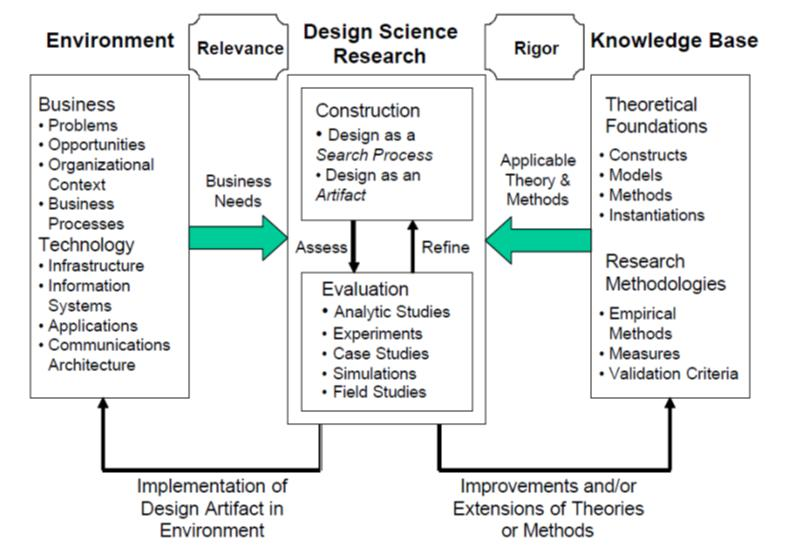
\includegraphics[width=0.7\linewidth]{./img/InformationSystemResearchFramework.jpg}
	\caption{The Information System Research Framework as designed by \cite{hevner2010design}}
	\label{fig:InformationSystemResearchFramework}
\end{figure}

In this research, a case-study is done to check the working of negotiation in this new MAS framework. By comparing the model with a real-world situation, the new MAS framework can be assessed and maybe refined. Furthermore, it can be determined whether this negotiation method can be used in business context.

\section{Research Process}
Firstly a literature research was concluded to assess the current negotiation methods in agent manufacturing systems. Afterwards a mapping of the processes, clarification of the objectives and determination of the requirements related to the use-case was performed. It was important to define the boundaries of the context system and the evaluation method before the system was built. From the literature a knowledge gap is found, which could be used in future manufacturing processes.

Based on this knowledge gap, a mathematical model, to assess how the negotiation will concur in the multi-agent system, will be created. A simulator will be created to evaluate this method. After the creation of the model and simulator, the relevance will be assessed by its performance.

%After the creation of the model and simulator, the relevance will be assessed by performing business analytic's. This will be done in the form of interviews on which business opportunities can be assessed.

The operational requirements should be clear then, and the theory can match the business expectations. From this, future prospects can be concluded.


%\todo{How to evaluate }
\subsection{Evaluation Method}
%\Todo{Alignen met de rest van de introductie text}
To test the final theoretical framework, a virtual simulation is to be created. The agents will be shown, including their desire, and for example their knowledge. In such a simulation, the negotiation can be visualized, and proof for the (near-)optimal outcome can be shown. 

Depending on the eventual data source, two evaluation methods are possible. If a ``real'' data source is available, the Key Performance Indicator (KPI) of the business will be checked. By minimizing e.g. the consumed base and acid during the production process, an improvement of the new system can be concluded.

If a ``real'' data source cannot be found, the model is to be evaluated using the known Nash solution. Since we know the optimal solution of the group we can determine the effectivity of the method, and evaluated the model in aspects of speed, quality solution, and dynamicity.

\section{Research Questions}
From the research goals and process, the following research questions are concluded:
\begin{enumerate}
	\item
	How can energy and manufacturing companies use the AI concept of intelligent multi-agent systems (MAS) for the optimization of production planning incl predictive maintenance and/or process control optimization?
	\begin{enumerate}
		\item
		What is the optimal MAS framework for the optimization of production planning?
		\begin{enumerate}
			\item 
			Theoretical: Which negotiation techniques, communication protocols, knowledge models and hierarchy/coalition to optimize decision making/scheduling.
			\item
			Simulation: Compare the new framework to an old use-case using simulation results.
		\end{enumerate}
		%\item
		%What are the technical requirements for such a system?
		%\begin{enumerate}
		%	\item
		%	Internet of Things: Sensors, protocol, Industry 4.0
		%\end{enumerate}
		\item
		What is the Framework for other industries within the industry 4.0?
		\begin{enumerate}
			\item 
			Decentralized systems vs Centralized systems
			\item
			Negotiation in manufacturing
		\end{enumerate}
	\end{enumerate}
\end{enumerate}

